\chapter{Decision trees}

Decision tree learning is one of the predictive modeling approaches used in machine learning. It uses a decisione tree as a predictive model to go from observations about an item (represented in the branches) to conclusions about the item's target value (represented in the leaves). Tree models where the target variable can take a discrete set of values are called \textbf{classification trees}; in these tree structures, leaves represent class labels and branches represent conjunctions of features that lead to those class labels. Decision trees where the target variable can take continuous values are called \textbf{regression trees}. Decision trees are among the most popular machine learning algorithms given their intelligibility and simplicity.

\begin{wrapfigure}{r}{0.25\textwidth}
    \begin{center}
        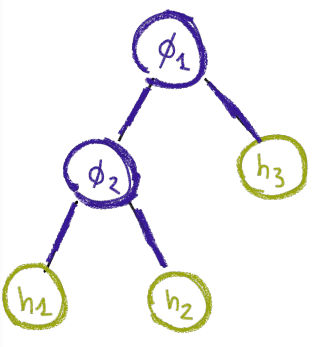
\includegraphics[width=0.25\textwidth]{033}
        \label{fig:033}
    \end{center}
    \caption{}
    \vspace{-40pt}
\end{wrapfigure}

A decision tree is a non-parametric supervised learning algorithm, it has a hierarchical tree structure, which consists of a root node, branches, internal nodes, and leaf nodes. The concept of a decision tree is to select splits that decrease the impurity of class distribution in the resulting subsets of instances. At the same time, the domination of one or more classes over the other classes is increased. This way, you can find a subset that contains only instances of one class after a few splits. For decision trees, binary trees are referred because they can be generalized better than trees with high-cardinality attributes.

\section{How decision trees work}
A decision tree starts with a root node, which does not have any incoming branches. The outgoing branches from the root node then feed into the internal nodes, also knows as \textbf{decision nodes}. Based on the available features, both node types conduct evaluations to form homogeneous subsets, which are denoted by leaf nodes, or terminal nodes. The leaf nodes represent all the possible outcomes within the dataset.

A decision tree takes an input \(x \in X\), the growing starts from a single root node, and routes it through its nodes until it reaches a leaf node. Each non-terminal node \(Node(\phi, t_L, t_r)\) holds a routing function \(\phi \in \{L,R\}^X\), a left child \(t_L\) and a right child \(t_R\). When \(x\) reaches the node it will go to the left child \(t_L\) or the right child \(t_R\) depending on the value of \(\phi(x) \in \{L,R\}\). When you do a split, each of the created descendant nodes corresponds to the applicable subset of the training data set. Further splits of these nodes result in new nodes that correspond to smaller subsets of data sets, and so on. Nodes that are not split further become leaves, each leaf node \(Leaf(h)\) holds a prediction function \(h \in F_\text{task}\) (typically a constant), depending on the task we want to solve it can be \(h \in Y^X\) (classification or regression) or \(h \in \Delta(X)\) (density estimation) or other. Once \(x\) reaches the leaf, the final prediction is given by \(h(x)\).

Decision tree learning employs a divide and conquer strategy by conducting a greed search to identify the optimal split points within a tree. this process of splitting is then repeated in a top-down, recursive manner until all, or the majority of records have been classified under specific class labels.

\subsubsection{Inference}
In order to infer with the decision tree, we define \(f_t\), the function returning the prediction for input \(x \in X\) according to the decision tree \(t\), that is recursively defined as
\begin{equation}
    f_t(x) = \begin{cases}
        h(x)                 &\text{if } t = Leaf(h)\\
        f_{t_{\phi(x)}}(x)   &\text{if } t = Node(\phi,t_L,t_R)\\
    \end{cases}
\end{equation}
Namely, given an input sample \(x\), if the decision tree \(t\) is a leaf, then do the prediction \(h(x)\); otherwise, if the decision tree \(t\) is a node, then call recursively the prediction function \(f\) on the left decision tree node \(t_L\) or right decision tree node \(t_R\), depending on the value of the function \(\phi(x)\).

\section{Decision tree learning algorithm}
\begin{figure}[t]
\begin{center}
    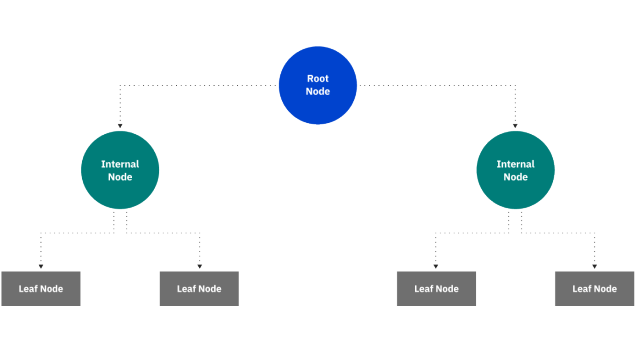
\includegraphics[width=0.75\textwidth]{098}
\end{center}
\caption{Decision tree structure.}
\label{fig:098}
\end{figure}
Given a training set \(D_n=\{z_1,...,z_n\}\), the set \(T\) of all the possible decision trees, find \(f_{t^*}\), that corresponds to the optimal tree, where 
\begin{equation}
    t^* \in arg\ \min_{t \in T} E(f_t;D_n)
\end{equation}
The optimization problem is easy if we don't impose constraints (e.g. most compact tree), a solution can be found using a simple, greedy strategy. Otherwise, the complexity class could be NP-hard. Hereafter, we will assume:
\begin{equation}
    E(f_t; D) = \frac 1 {|D|} \sum_{z \in D} l(f;z)
\end{equation}
That means that the empirical error of our training set can be computed by the normalized sum of the pair-wise losses.

Fix a set of leaf predictions \(H_\text{leaf} \subset F_\text{task}\) (e.g., constant functions), that correspond to the number of classes. Fix a set of possible split functions \(\Phi \subset \{L,R\}^X\). Define the tree-growing strategy that recursively partitions the training set and decides whether to grow leaves or non-terminal nodes. Finally, we stop when the final criteria is reached, and all the examples of the current training set are associated to the same class. 

\subsubsection{Growing a leaf}
Growing a leaf means to find a way to know if the current training set are associated to the same class. Formally, given \(D = \{z_1,...,z_n\}\) the training set reaching the node. The optimal leaf predictor, that minimizes the local error, can be computed as:
\begin{equation}
    h_D^* \in arg \min_{h \in H_\text{leaf}} E(h;D)
\end{equation}
The optimal error value is also called \textbf{impurity measure}, and tells us what is the probability of misclassifying an observation. Note that the lower the impurity, the better the split.
\begin{equation}
    I(D) = E(h_D^*; D)
\end{equation}
If some criterion is met we grow a leaf \(Leaf(h_D^*)\), for example:
\begin{itemize}
    \item 
    Purity \(I(D) < E\);
    \item
    Minimum cardinality \(|D| < k\);
    \item
    Others...
\end{itemize}

\subsubsection{Growing a node}
Given the set of all the possible routing functions \(\Phi\), and the set of training samples \(D\); if no stopping criterion is met, find the optimal split function, by minimizing the impurity function of our training set.
\begin{equation}
    \phi_D^* \in arg\ \min_{\phi \in \Phi} I_\phi (D)
\end{equation}
The impurity \(I_\phi(D)\) of a split function \(\phi\) given a training set \(D\) is computed in terms of the impurity of the split data:
\begin{align}
    I_\phi(D) &= \sum_{d \in \{L,R\}} \frac {|D_d^\phi|} {|D|} I(D_d^\phi)\\
    D_d^\phi &= \{(x,y) \in D; \phi(x) = d\}
\end{align}
Note that the impurity of a split function is the lowest training error that can be attained by a tree consisting of a root and two leaves.

Now, we finally grow a node \(Node(\phi^*, t_L, t_R)\), where \(\phi^*\) is the optimal split. \(t_L\) and \(t_R\) are obtained by recursively applying the learning algorithm to the associated training set splits.

In a nutshell:
\begin{equation}
    \text{Grow}(D)=\begin{cases}
        Leaf(h_D^*)                                                &\text{if stopping criterion met}\\
        Node(\phi_D^*, \text{Grow}(D_L^*), \text{Grow}(D_R^*))     &\text{otherwise}
    \end{cases}
\end{equation}

\subsection{About split selection}
Sometimes the selection of the best split function is not given in terms of minimizing the impurity of the split, but in the equivalent maximization of information gain, which is given by:
\begin{equation}
    \Delta_\phi(D)=I(D)-I_\phi(D)
\end{equation}
Information gain is non-negative, i.e. \(\Delta_\phi(D) \geq 0\) for any \(\phi \in \{L,R\}^X\) and any training set \(D \subset X \times Y\). So, the impurity will never increase for any randomly chosen split.

\subsection{Leaf predictions}
The leaf rediction provides a solution to a simplified problem involving only data reaching the leaf. This solution can be an arbitrary function \(h \in F_\text{task}\) but in practice we restrict it to a subset \(H_\text{leaf}\) of simple ones. 

The simplest predictor one can construct is a function returning a constant (e.g. a prefixed class label). The set of all possible constant functions can be written as:
\begin{equation}
    H_\text{leaf} = \bigcup_{y \in Y} \{y\}^X
\end{equation}

\section{Impurity measures for classification}
The impurity is a measure to take care of, because it can completely change the construction of the decision tree: the decision trees decide whether a node can be an inner node or a leaf, based on the impurity measure, which makes critical the decision of the kind of measure to choose for the model.

In the case of classification, we have an output space \(Y = \{c_1,...,c_k\}\) and a training set \(D \subset X \times Y\), that is the cartesian product of the input space and output space. Let \(D^y = \{(x,y') \in D : y = y'\}\) denote the subset of training samples in \(D\) with class label \(y\). 

Consider the following error function:
\[E(f;D) = \frac 1 {|D|} \sum_{z \in D} l(f;z)\]
With respect to this equation, we can now have different loss function that can lead us to completely different error functions.

\subsubsection{Classificationn error}
If the loss function is \(l(f;(x,y)) = 1_{f(x) \neq y}\), meaning that it is \(1\) if the condition \(f(x) \neq y\) is verified, and \(H_\text{leaf} = \cup_{y \in Y} \{y\}^X\), where \(H_\text{leaf}\) is the set of all the leaves, then the impurity measure is the misclassification rate, or \textbf{classification error}:
\begin{equation}
    I(D) = 1 - max_{y\in Y} \frac {|D^Y|} {|D|}
\end{equation}

\subsubsection{Gini Impurity}
If the set of all the leaves is \(H_\text{leaf} = \cup_{\pi \in \Delta(Y)} \{\pi\}^X\), that is the constaint label distribution as leaf prediction, and the loss function is \(l(f;(x,y)) = \sum_{c \in Y} [f_c(x) - 1_{c=y}]^2\), then the impurity measure is the \textbf{Gini impurity}:
\begin{equation}
    I(D) = 1 - \sum_{y \in Y} \left( \frac {|D^y|} {|D|} \right) ^2
\end{equation}
The Gini impurity is a measure of how often a randomly chosen element from the set would be incorrectly labeled if it was randomly labeled according to the distribution of labels in the subset.

\subsubsection{Entropy}
In data science, the entropy is used as a way to measure the level of disorder, and can give a deterministic value of how mixed a column is, that is the information. The more mixed our set of all leaves is, the higher the entropy, so we can use the formula to determine how good the split has been.

If the set of all the leaves is again defined as the constant label distribution \(H_\text{leaf} = \cup_{\pi \in \Delta(Y)} \{\pi\}^X\), and the loss function is defined as \(l(f;(x,y)) = -\log f_y(x)\) then the impurity measure is the \textbf{entropy}:
\begin{equation}
    I(D) = - \sum_{y \in Y} \frac {|D^y|} {|D|} \log \frac {|D^y|} {|D|}
\end{equation}

\section{Impurity measures for regression}
In the case of regression, we have the output space \(Y \subset \mathbb(R)^d\), and \(D \subset X \times Y\). If \(l(f;(x,y)) = ||f(x) - y||^2\), and \(H_\text{leaf}=\cup_{y \in Y} \{y\}^X\), then the impurity measure is the \textbf{variance} associated to all the points in the  training set:
\begin{equation}
    I(D) = \frac 1 {|D|} \sum_{(x,y) \in D} ||x - \mu_D||^2
\end{equation}
where \(\mu_D = \frac 1 {|D|} \sum_{(x,y) \in D} x\) is the \emph{mean} of all the points in the training set.

\section{Split functions}
A data point \(x \in X\) could be \(d\)-dimensional with each dimension taking heterogeneous types of values (discrete, continuous) and have a total ordering or not (ordinal or nominal).

The split function \(\phi \in \{L,R\}^X\) determines wheter a data point \(x \in X\) should move left (\(\phi(x) = L\)) or right (\(\phi(x) = R\)). The possible split functions are restricted to some predefined set \(\Phi \subset \{L,R\}^X\) depending on the nature of the feature space. The prototypical split function for a \(d\)-dimensional input first selects one dimension and then applies a \(1\)-dimensional splitting criterion.

\subsection{Discrete nominal features}
Assume discrete nominal features taking values in \(K\) (e.g. colors, marital status, etc.). The split function can be implemented given a partition of \(K\) into \(K_R\) and \(K_L\), associated to different partitions of the tree.
\begin{equation}
    \phi(x) = \begin{cases}
        L \qquad &\text{if }x \in K_L \\
        R \qquad &\text{if }x \in K_R \\
    \end{cases}
\end{equation}
Finding the optimal split requires testing \(2^{|K|-1}-1\) bi-partitions.

\subsection{Ordinal features}
Assume ordinal features, i.e. can be sorted (numbers, t-shirt sizes, etc.), taking values in \(K\). The split function can be implemented given a threshold \(r \in K\):
\begin{equation}
    \phi(x) = \begin{cases}
        L \qquad &\text{if }x \leq r \\
        R \qquad &\text{if }x > r \\
    \end{cases}
\end{equation}
If \(|K| \leq |D|\), finding the optimal split requires testing \(|K|-1\) thresholds. Otherwise, it requires sorting the input values in \(D\), where \(D\) is the training set reaching the node, and testing \(|D|-1\) thresholds.

\subsection{Oblique}
Sometimes it is convenient to split using multiple features at once. Such split functions work with continuous features and are called \textbf{oblique}, because can generate oblique decision boundaries. If \(x \in \mathbb{R}^d\) then the split function can be implemented given \(w \in \mathbb{R}^d\) and \(r \in \mathbb{R}\):
\begin{equation}
    \phi(x) = \begin{cases}
        L \qquad &\text{if }w^Tx \leq r \\
        R \qquad &\text{otherwise} \\
    \end{cases}
\end{equation}

\section{Overfitting}
Decision trees are \textbf{non-parametric models} with a structure that is determine by the data. As a result, they are flexible and can wasily fit the training set, but with high risk of \textbf{overfitting}. 

Standard techniques to improve generalization apply also to decision trees:
\begin{itemize}
    \item early stopping;
    \item regularization;
    \item data augmentations;
    \item complexity regularization;
    \item ensembling.
\end{itemize}

\subsection{Pruning}
Pruning is a data compression technique that reduces the size of decision trees by removing sections in the tree that are non-critical and redundant to classify instances. Pruning reduces the complexity of the final classifier, and hence improves predictive accuracy by the reduction of overfitting.

A common strategy is to grow the tree until each node contains a small number of instances then use pruning to remove nodes that do not provide additional information.

Pruning should reduce the size of a learning tree without reducing predictive accuracy as measured by a cross-validation set. There are many techniques for tree pruning that differ in the measurement that is used to optimize performance.

\section{Random forests}
Random forests are an ensemble learning method for classification, regression, and other tasks that operate by constructing a multitude of decision trees at training time. For classification tasks, the output of the random forest is the class selected by most trees. For regression tasks, the mean or average prediction of the individual trees is returned. Random forests correct for decision trees' habit of overfitting to their training set. They generally outperform decision trees, but their accuracy is lower than gradient boosted trees. However, data characteristics can affect their performance. 

If we build many trees, all of which work weel and overfit in different ways, we can reduce the amount of overfitting by averaging their results. This reduction in overfitting, while retaining the predictive power of the trees, can be shown using rigorous mathematics.

To implement this strategy, we need to build many decision trees. Each tree should do an acceptable job of predicting the target, and should also be different from the other trees. Random forests get their name from injecting randomness into the tree building to ensure each tree is different.

Split functions are optimized on randomly sampled features, or are sampled completely at random. This helps obtaining decorrelated decision trees. The final prediction of the forest is obtained by averaging the prediction of each tree in the ensemble \(Q = \{t_1,...,t_T\}\).
\begin{equation}
    f_Q(x) = \frac 1 T \sum_{j=1}^T f_t(x)
\end{equation}

\subsection{Algorithm}
\begin{algorithm}
\caption{Random Forest Learning}
\label{alg:perceptron}
\ForEach{$b \gets 1$ to $B$}{
    Draw a boostrap sample $\vec{Z}^*$ of size $N$ from the training data\;
    Grow a random-forest tree $T_b$ to the bootstrapped data\;
    \ForEach{terminal node of $T_b$}{
        \Repeat{minimum node size $n_\min$ is reached}{
            Select $m$ variables at random from the $p$ variables\;
            Pick the best variable/split-point among the $m$\;
            Split the node into two daughter nodes\;
        }
    }
}
\Return{Output the ensemble of trees ${\{T_b\}^B}_1$}
\end{algorithm}

While random forests often achieve higher accuracy than a single decision tree, they sacrifice the intrinsic interpretability present in decision trees. They are very powerful, often work well without heavy tuning of the parameters, and don't require scaling of the data. Essentially, they share all of the benefits of decision trees, while making up for some of their deficiencies.

\begin{figure}[b!]
\begin{center}
    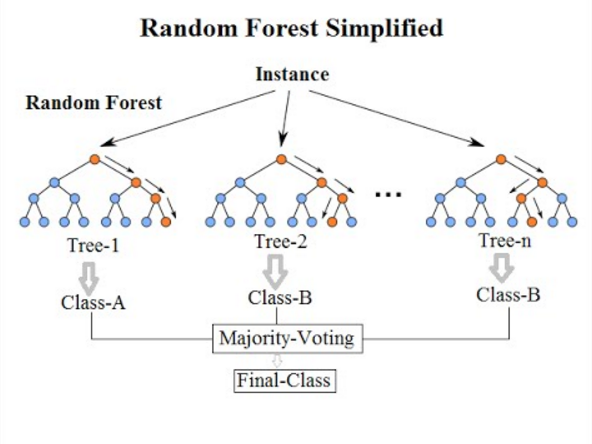
\includegraphics[width=.75\textwidth]{034}
\end{center}
\caption{Random forest classification example}
\label{fig:034}
\end{figure}

One reason to still use decision trees is if you need a compact representation of the decision making process. It is basically impossible to interpret tens or hundreds of trees in detail, and trees in random forests tend to be deeper than decision trees.

One application example of the random forest is a notable application in computer vision: the \textbf{kinect}.

\newpage
\begin{exercise}[topsep=20pt,itemsep=10pt]
    \ex Describe the decision trees. How does a decision tree work?
    \ex How does a decision tree infer?
    \ex[!] Describe the decision tree learning algorithm.
    \ex[!] How does a decision tree know when to grow a leaf and when to grow an inner node?
    \ex Describe the classification error, the Gini impurity, and the entropy.
    \ex Describe the split function for discrete nominal features, ordinal features.
    \ex What is the oblique? 
    \ex How can the overfitting problem solved? Describe the concept of pruning.
    \ex Describe the random forests. What are the differences with respect to decision trees?
    \ex[!] What are the advantages of random forests against decision trees?
\end{exercise}